\section{Start Inviwo and run ENVISIoN scripts}

\\
If the user wishes to run Inviwo with its own graphical user interface, it's possible and still have access to the visualizations provided by ENVISIoN. These visualizations are stored in the form of Python scripts that can be compiled through the Inviwo user interface.

To run Inviwo in an UNIX environment, execute the commands below.

\begin{lstlisting}[frame = single, breaklines=true]
cd ENVISIoN/ENVISIoN
 ./inviwo-build/bin/inviwo
\end{lstlisting}

When the Inviwo interface has opened, follow the instructions given in figure \ref{fig:Inviwo} and in the list below to run a visualization script.

\begin{enumerate}
\item Locate and press the Python menu in the Inviwo bar.
\item Open the Python editor by pressing it.
\item In the Python editor, click Open Script.
\item Select one of the scripts. The ENVISIoN scripts can be located in \emph{$\sim$/ENVISIoN/scripts}.
\item Click open.
\item Click the button in the top left corner to run.
\end{enumerate}

\begin{figure}[ht]
    \centering
    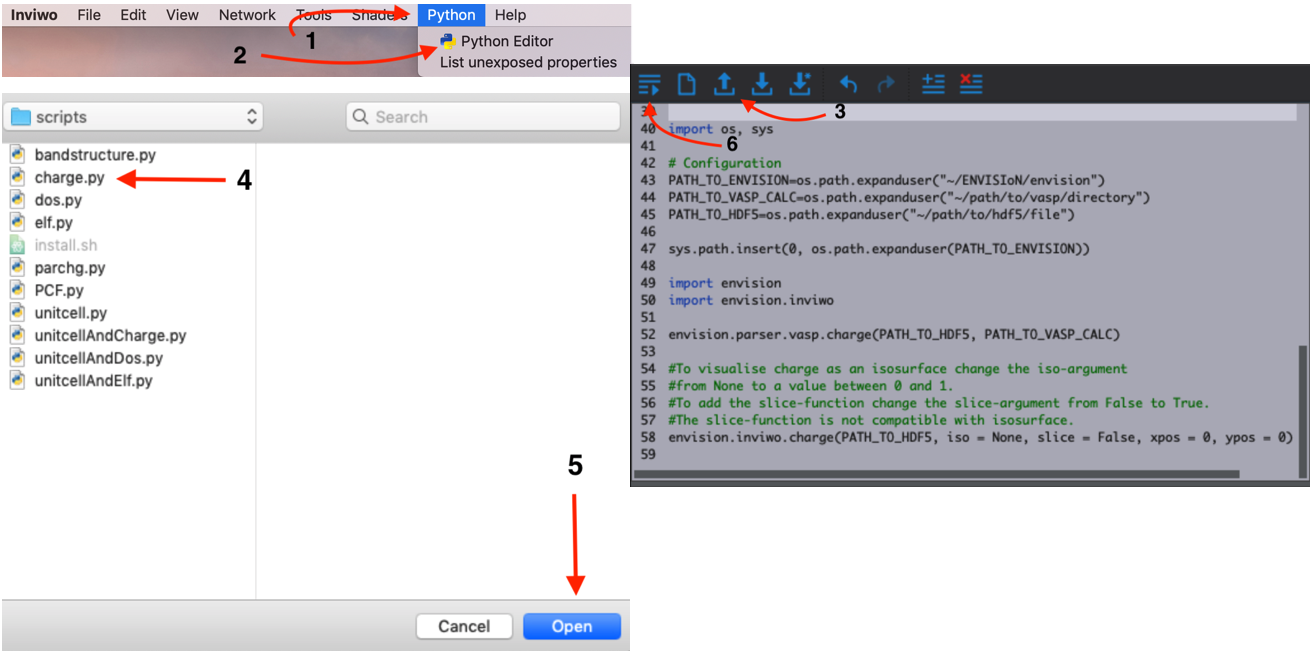
\includegraphics[angle=0, width=\linewidth]{images/completeInviwo.png}
    \caption{Cutout from Inviwo with instructions on how to run a ENVISIoN visualization script in numeric order.}
    \label{fig:Inviwo}
\end{figure}
